\subsubsection{Jupyter Magic Commands}

\newline
In addition to running Python code, Jupyter Notebooks provide magic commands with various functions. We provide an introduction to a several, but many more are available. Plese see the \href{https://ipython.readthedocs.io/en/stable/interactive/magics.html}{Jupyter Magics documentaion} for more information.

\begin{itemize}
\item Shell~Assignment~Syntax
\item Line~Magics
\item Cell~Magics
\end{itemize}


\bigskip
\centerline{\rule{13cm}{0.4pt}}
\bigskip

\paragraph{Shell Assignment Syntax}\label{Shell-Assignment-Syntax}

In Jupyter Notebooks, the exclamation mark \texttt{!} allows users to run shell commands from inside a Jupyter Notebook code cell (\texttt{/bin/bash} in OpenSARLab).

Simply start a line of code with \texttt{!} and it will run the command in a shell, using the Conda environment of the currently running Python kernel.

\begin{figure}[!htbp]
\centering
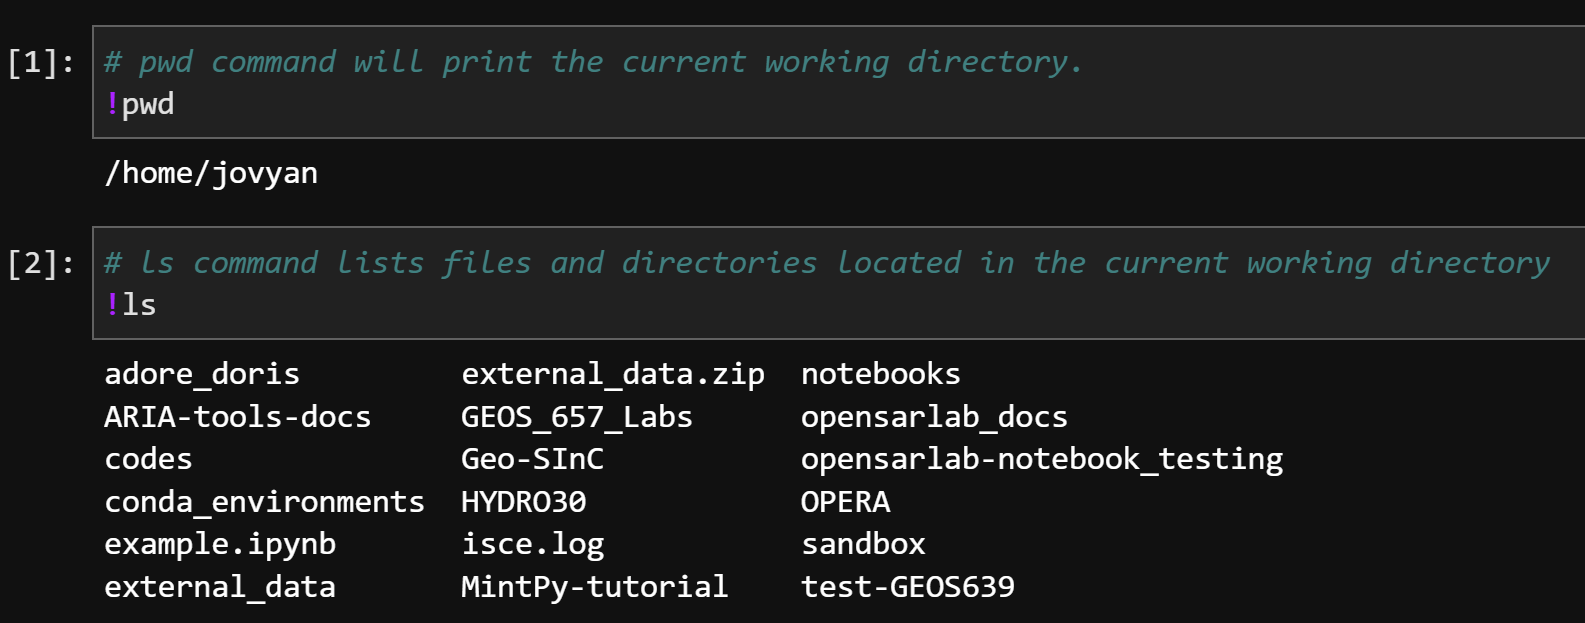
\includegraphics[width=0.7\linewidth]{files/magic_excl-12ba8e58141a58cf8b7fc5b21fa3c978.PNG}
\caption*{Using \texttt{!} to run shell commands in a Jupyter Notebook.}
\end{figure}


\bigskip
\centerline{\rule{13cm}{0.4pt}}
\bigskip

\paragraph{Line Magics}\label{Line-Magics}

Line magics start with a single \texttt{\%}. They either update a setting that affect the entire notebook or they affect only the line where \texttt{\%} is used.

\subparagraph{\texttt{\%matplotlib inline}}

\begin{itemize}
\item Display \textbf{non-interactive} \texttt{matplotlib plots} in code cell output.
\item Turns on inline plotting for the entire notebook
\end{itemize}

\subparagraph{\texttt{\%matplotlib widget}}

\begin{itemize}
\item Display \textbf{interactive} \texttt{matplotlib plots} in code cell output.
\item Turns on interactive plotting for the entire notebook.
\end{itemize}

\subparagraph{\texttt{\%time}}

\begin{itemize}
\item Time the execution of a Python expression.
\item Times only the line containing the \texttt{\%time} magic command.
\end{itemize}

\subparagraph{Find information on many more line magics \href{https://ipython.readthedocs.io/en/stable/interactive/magics.html\#:~:text=IPython\%20trove\%20classifier.-,Line\%20magics,-\%EF\%83\%81}{here}.}


\bigskip
\centerline{\rule{13cm}{0.4pt}}
\bigskip

\paragraph{Cell Magics}\label{Cell-Magics}

Cell magics start with \texttt{\%\%} and affect the contents of an entire code cell.

\subparagraph{\texttt{\%\%javascript} or \texttt{\%\%js}}

\begin{itemize}
\item Run a JavaScript code cell.
\end{itemize}

\begin{figure}[!htbp]
\centering
\includegraphics[width=0.7\linewidth]{files/magic_js-c34fba5a522f55637fc0723db6ae7d55.gif}
\caption*{Jupyter Javascript magic example.}
\end{figure}

\subparagraph{\texttt{\%\%capture}}

\begin{itemize}
\item Run a code cell but capture and hide all output.
\end{itemize}

\subparagraph{Find information on many more cell magics \href{https://ipython.readthedocs.io/en/stable/interactive/magics.html\#cell-magics:~:text=True\%20value\%20set.-,Cell\%20magics,-\%EF\%83\%81}{here}.}